\chapter{State of the Art}
\graphicspath{{state-of-the-art/figures/}}

In recent years, the remarkable advancements in Natural Language Processing (NLP) have been primarily driven by the development of LLMs. These LLMs, such as GPT (Generative Pretrained Transformer) and BERT (Bidirectional Encoder Representations from Transformers), have demonstrated remarkable capabilities in understanding and generating human-like text. However, despite their impressive performance, LLMs still face challenges in effectively retrieving and incorporating relevant context for generating accurate and coherent responses.

Enter RAG systems, a novel approach that seeks to overcome the limitations of traditional LLMs by integrating retrieval mechanisms with generation models. RAG systems combine the strengths of both retrieval and generation techniques to enhance the quality and relevance of generated text.

This chapter provides a comprehensive exploration of RAG systems, delving into their architecture, components, training processes, applications, advantages, and challenges. We begin by establishing a foundational understanding of LLMs and their evolution, laying the groundwork for understanding the need for RAG systems. We then proceed to dissect the intricacies of RAG systems, discussing the role of retrieval in providing context and the role of generation in producing fluent responses.

Through detailed examination and analysis, we uncover the inner workings of RAG systems, exploring how retrieval and generation components interact within the architecture. Real-world applications and use cases of RAG systems across various domains are elucidated, demonstrating their potential to revolutionize tasks such as question answering, dialogue generation, and content creation.

Furthermore, we evaluate the advantages and limitations of RAG systems compared to traditional LLMs and other approaches in NLP. By examining performance metrics, challenges, and future directions, we gain insights into the transformative impact of RAG systems on the field of natural language processing.

In summary, this chapter serves as a comprehensive guide to RAG systems, offering readers a deep dive into one of the most promising advancements in NLP. As we navigate through the complexities and potentials of RAG systems, we pave the way for understanding their role in shaping the future of human-computer interaction and language understanding.

\section{Machine Learning}

\subsection{Definition}


Machine Learning, often abbreviated as ML, is a subset of artificial intelligence (AI) that focuses on the development of computer algorithms that improve automatically through experience and by the use of data. In simpler terms, machine learning enables computers to learn from data and make decisions or predictions without being explicitly programmed to do so.

At its core, machine learning is all about creating and implementing algorithms that facilitate these decisions and predictions. These algorithms are designed to improve their performance over time, becoming more accurate and effective as they process more data.

In traditional programming, a computer follows a set of predefined instructions to perform a task. However, in machine learning, the computer is given a set of examples (data) and a task to perform, but it's up to the computer to figure out how to accomplish the task based on the examples it's given.

For instance, if we want a computer to recognize images of cats, we don't provide it with specific instructions on what a cat looks like. Instead, we give it thousands of images of cats and let the machine learning algorithm figure out the common patterns and features that define a cat. Over time, as the algorithm processes more images, it gets better at recognizing cats, even when presented with images it has never seen before.

This ability to learn from data and improve over time makes machine learning incredibly powerful and versatile. It's the driving force behind many of the technological advancements we see today, from voice assistants and recommendation systems to self-driving cars and predictive analytics \cite{datacamp:ml}.

\subsection{Relationships to other fields}

Artificial Intelligence (AI) encompasses the field of computer science dedicated to creating systems capable of emulating human-like intelligence, problem-solving, and decision-making. Machine Learning (ML) is a subset of AI focused on enabling computers to learn from data without being explicitly programmed. Within ML, Deep Learning stands out as a subfield that employs neural networks with multiple layers to learn complex representations of data, particularly effective in tasks like image and speech recognition. ML and Deep Learning are integral components of AI, providing the framework for developing intelligent systems capable of learning, reasoning, and adapting to new information, thereby advancing the capabilities of AI across various domains.

\begin{figure}[htpb]
    \centering
    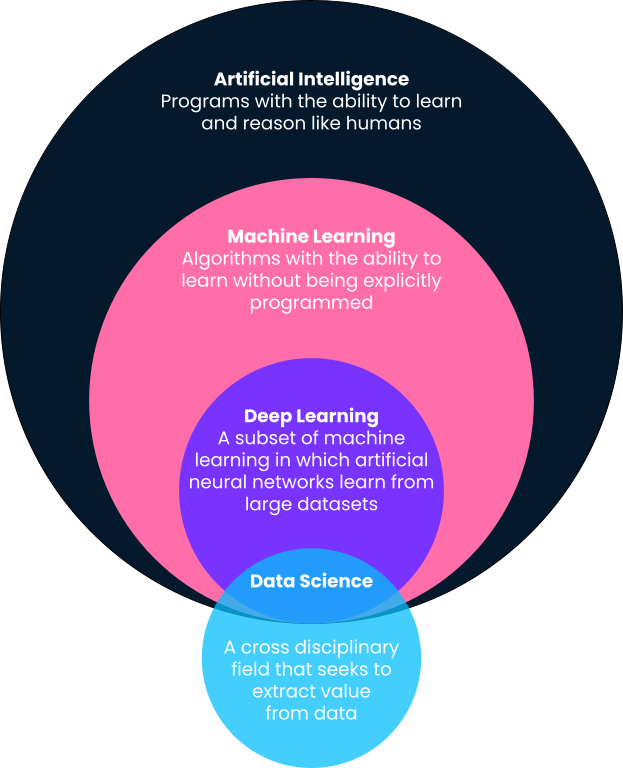
\includegraphics[width=\textwidth,height=6cm,keepaspectratio=true]{ml.png}
    \caption{
        Machine learning as subfield of AI, from \cite{datacamp:ml}.
    }
\end{figure}

\subsection{Types of Machine Learning}

Machine Learning can be broadly categorized into several types based on the learning approach, the availability of labeled data, and the feedback mechanism. The main types of machine learning are:

\begin{figure}[htpb]
    \centering
    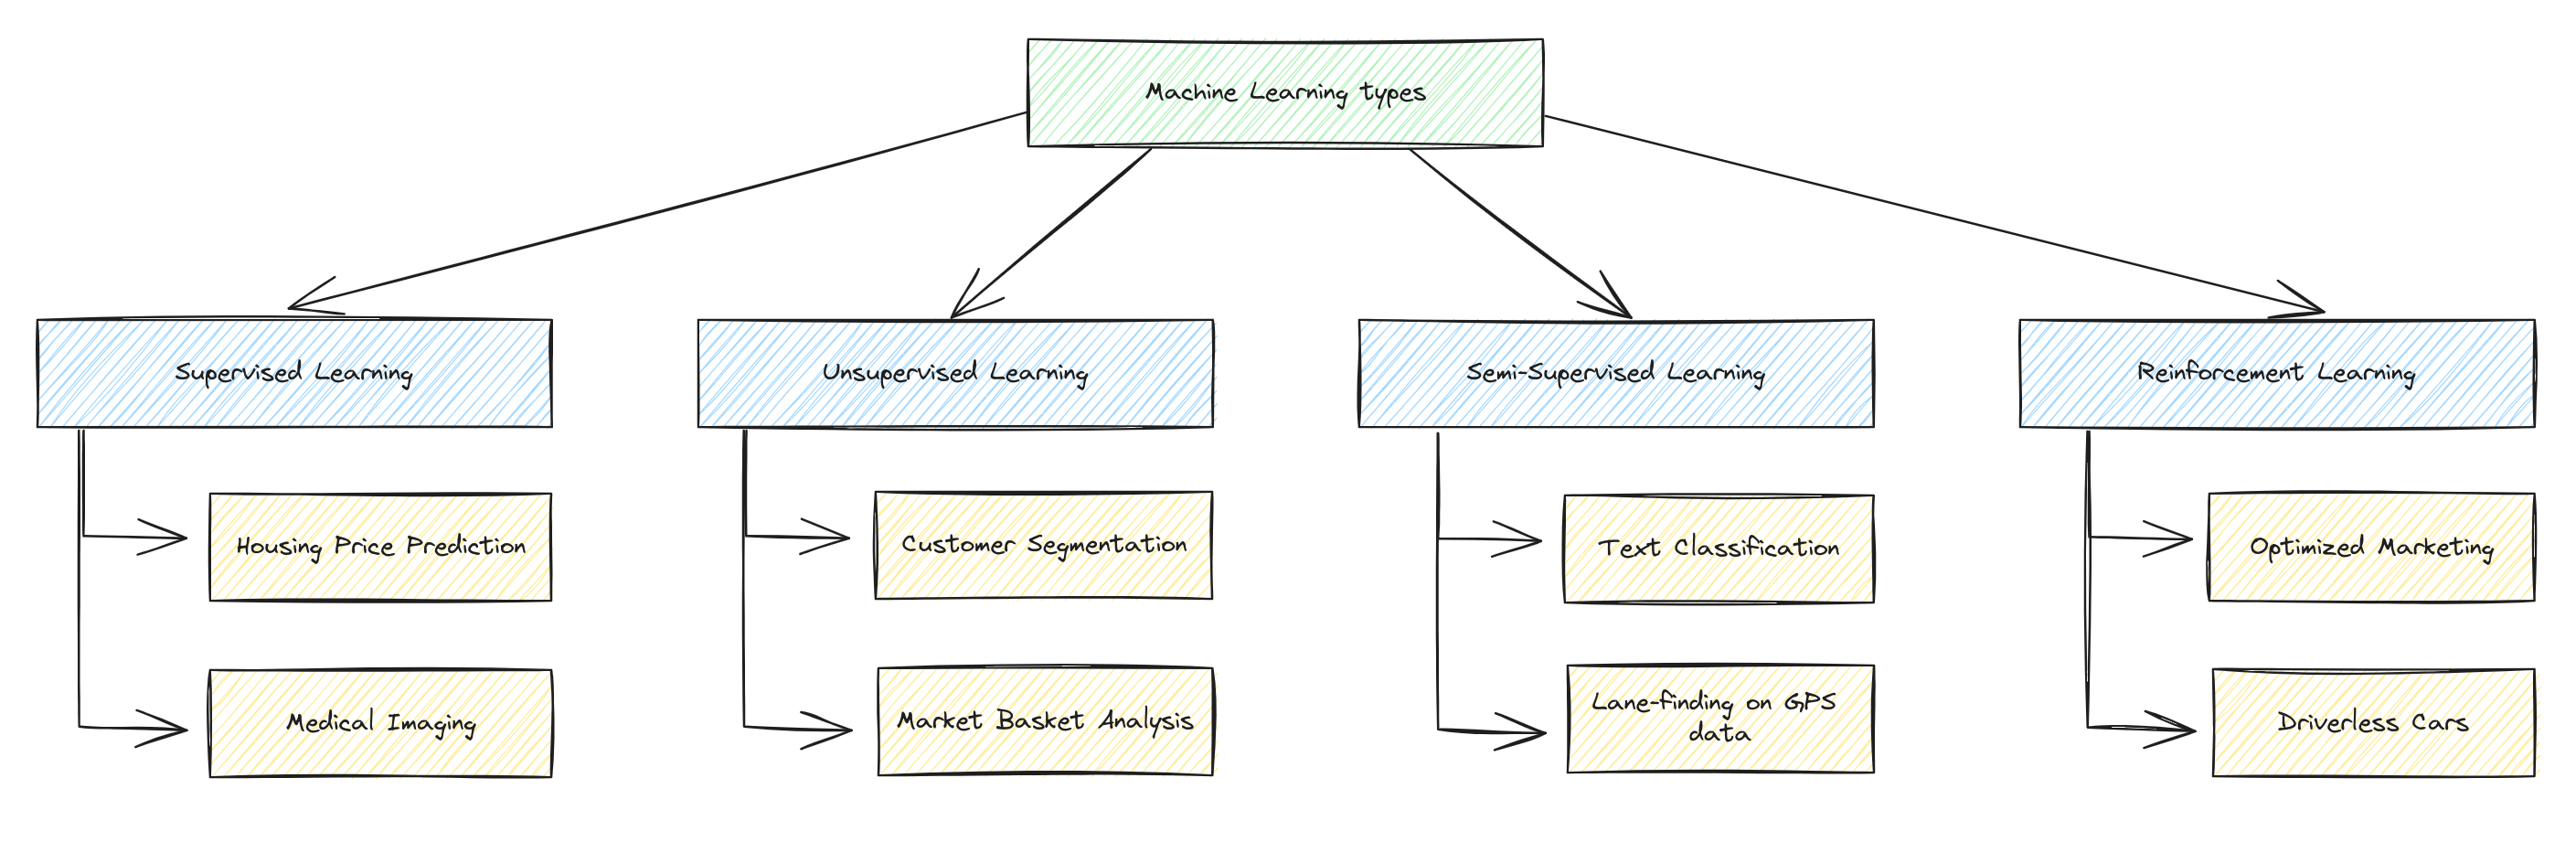
\includegraphics[width=\textwidth,height=6cm,keepaspectratio=true]{ml-types.png}
    \caption{
        Types of machine Learning.
    }
\end{figure}

\subsubsection*{Supervised Learning}

\begin{itemize}
    \item{In supervised learning, the algorithm learns from labeled data, where each input example is paired with the corresponding output label.}
    \item{The goal is to learn a mapping from inputs to outputs, allowing the algorithm to make predictions or classifications on unseen data.}
    \item{Common supervised learning tasks include regression (predicting continuous values) and classification (predicting discrete labels).}
\end{itemize}

\subsubsection*{Unsupervised Learning:}

\begin{itemize}
    \item{Unsupervised learning involves learning from unlabeled data, where the algorithm aims to find patterns, structures, or relationships in the data without explicit guidance.}
    \item{The algorithm discovers hidden structures or clusters within the data, facilitating tasks such as clustering, dimensionality reduction, and anomaly detection.}
\end{itemize}

\subsubsection*{Semi-Supervised Learning:}

\begin{itemize}
    \item{Semi-supervised learning lies between supervised and unsupervised learning, where the algorithm learns from a combination of labeled and unlabeled data.}
    \item{The presence of both labeled and unlabeled data allows the algorithm to leverage additional information and improve performance, particularly in scenarios where labeled data is scarce or expensive to obtain.}
\end{itemize}

\subsubsection*{Reinforcement Learning:}

\begin{itemize}
    \item{Reinforcement learning involves an agent learning to make decisions by interacting with an environment to achieve a specific goal.}
    \item{The agent receives feedback in the form of rewards or penalties based on its actions, enabling it to learn through trial and error.}
    \item{Reinforcement learning is commonly used in applications such as game playing, robotics, and autonomous systems.}
\end{itemize}

\subsection{Limitations of Machine Learning: Challenges and Considerations}

Although machine learning is a powerful technique for extracting knowledge from data, it also has certain limitations that are important to consider:

\begin{itemize}
    \item{\textbf{Data dependency:} Machine learning heavily relies on the quality and quantity of training data. If the data is poorly labeled or unrepresentative, it can lead to errors in predictions.}
    \item{\textbf{Overfitting:} When the model is too complex compared to the training data, it can overfit and not generalize well to test data. This can also result in poor performance for new data.}
    \item{\textbf{Explainability:} Machine learning models can be very complex and difficult to understand. It can be challenging to understand how the model makes decisions and to explain these decisions to users.}
    \item{\textbf{Biased data:} Training data can be biased due to factors such as data selection, human biases, or measurement errors. This can lead to biased predictions for test data.}
    \item{\textbf{Lack of diversity:} Machine learning models may lack diversity in the types of data they can handle. For example, machine learning models may struggle to process unstructured data such as images, sounds, and texts.}
    \item{\textbf{Computational cost:} Machine learning algorithms may require high computational power and significant storage resources to process large amounts of data. This can be costly and time-consuming to train and implement models.}
\end{itemize}


\section{Deep Learning}

\subsection{Definition}

Deep learning is a type of machine learning that teaches computers to perform tasks by learning from examples, much like humans do. Imagine teaching a computer to recognize cats: instead of telling it to look for whiskers, ears, and a tail, you show it thousands of pictures of cats. The computer finds the common patterns all by itself and learns how to identify a cat. This is the essence of deep learning.

In technical terms, deep learning uses something called "neural networks," which are inspired by the human brain. These networks consist of layers of interconnected nodes that process information. The more layers, the "deeper" the network, allowing it to learn more complex features and perform more sophisticated tasks \cite{datacamp:dl}.


\subsection{Deep Learning vs. Machine Learning}

Deep learning stands apart from traditional machine learning in its approach to data and learning methods.
Machine learning algorithms typically rely on structured, labeled data for predictions, where specific features are defined and organized into tables.
While machine learning can handle unstructured data, it often requires preprocessing to structure it. In contrast, deep learning streamlines this process by directly processing unstructured data such as text and images. It automates feature extraction, reducing reliance on human experts. For instance, in categorizing pet photos, deep learning algorithms autonomously identify key features, like ears, crucial for distinguishing between animals. In contrast, machine learning requires manual feature hierarchy establishment by human experts.

\subsection{Deep Learning Applications}

Deep learning has a wide range of applications across various domains due to its ability to learn complex patterns from large volumes of data. Some of the different types of applications for deep learning include:

\subsubsection*{Image Recognition and Computer Vision:}

\begin{itemize}
    \item Deep learning is extensively used for tasks such as image classification, object detection, facial recognition, and image segmentation.
    \item Applications include self-driving cars, medical image analysis, surveillance systems, and augmented reality.
\end{itemize}

\subsubsection*{Natural Language Processing (NLP):}

\begin{itemize}
    \item Deep learning is employed for understanding and generating human language, enabling tasks such as sentiment analysis, machine translation, text summarization, and chatbots.
    \item Applications include virtual assistants, language translation services, social media sentiment analysis, and customer support chatbots.
\end{itemize}


These are just a few examples of the diverse applications of deep learning, demonstrating its versatility and impact across various industries and fields.

\clearpage

\section{Natural Language Processing (NLP)}

Natural Language Processing (NLP) serves as a crucial technology within artificial intelligence, facilitating communication between humans and computers. It represents a multidisciplinary field empowering machines to comprehend, analyze, and produce human language, thus facilitating seamless human-machine interaction. The importance of NLP manifests in its diverse applications, spanning automated customer support to instantaneous language translation, showcasing its pivotal role in modern computing.

\subsection{What is Natural Language Processing?}

NLP emerges as a vital component within artificial intelligence, dedicated to facilitating communication between computers and humans via natural language. Its core objective lies in programming computers to effectively process and analyze extensive volumes of natural language data.

NLP encompasses the task of enabling machines to comprehend, interpret, and generate human language in a manner that is not only valuable but also meaningful. OpenAI, renowned for pioneering sophisticated language models such as ChatGPT, underscores the significance of NLP in fostering the development of intelligent systems capable of comprehending, responding to, and generating text. This advancement in technology serves to enhance user-friendliness and accessibility across various applications.

\subsection{How Does NLP Work?}

NLP is a fascinating field that delves into the intricate mechanisms underlying human language comprehension and generation by machines. This section aims to unravel the complexities of NLP, shedding light on the fundamental principles and techniques that drive its functionality. By exploring the inner workings of NLP, we gain insight into how machines process and analyze natural language data, paving the way for groundbreaking applications in artificial intelligence and human-computer interaction. Through this exploration, we embark on a journey to discover the algorithms, models, and methodologies that empower machines to navigate the vast landscape of human language with precision and sophistication.

\subsubsection*{Components of NLP}

Natural Language Processing is not a monolithic, singular approach, but rather, it is composed of several components, each contributing to the overall understanding of language. The main components that NLP strives to understand are Syntax, Semantics, Pragmatics, and Discourse.

\begin{itemize}
    \item \textbf{Syntax:} Syntax pertains to the arrangement of words and phrases to create well-structured sentences in a language.
    \item \textbf{Semantics:} Semantics is concerned with understanding the meaning of words and how they create meaning when combined in sentences.
    \item \textbf{Pragmatics:} Pragmatics deals with understanding language in various contexts, ensuring that the intended meaning is derived based on the situation, speaker's intent, and shared knowledge.
    \item \textbf{Discourse:} Discourse focuses on the analysis and interpretation of language beyond the sentence level, considering how sentences relate to each other in texts and conversations.
\end{itemize}

\subsubsection*{NLP techniques and methods}

NLP employs a diverse array of techniques and methodologies to analyze and comprehend human language. Below are some foundational techniques utilized in NLP:

\begin{itemize}
    \item \textbf{Tokenization:} This process involves segmenting text into individual units, such as words, phrases, or symbols, known as tokens.
    \item \textbf{Parsing:} Parsing entails examining the grammatical structure of a sentence to extract its meaning and syntactic relationships.
    \item \textbf{Lemmatization:} This technique involves reducing words to their base or root form, facilitating the grouping of different word forms with the same meaning.
    \item \textbf{Named Entity Recognition (NER):} NER is utilized to identify and classify entities within text, such as persons, organizations, locations, and other named items.
    \item \textbf{Sentiment Analysis:} This method enables the assessment of the sentiment or emotion expressed in a piece of text, aiding in understanding the underlying mood or opinion.
\end{itemize}

\subsubsection*{What is NLP Used For?}

With some of the basic concepts now defined, one can explore how natural language processing is applied in the modern world.

\begin{itemize}
    \item \textbf{Automatic Translation:} Automatic translation systems use NLP techniques to translate texts from one language to another.
    \item \textbf{Chatbots and Virtual Assistants:} Chatbots and virtual assistants use NLP to understand user's natural language and provide appropriate responses.
    \item \textbf{Automatic Summarization:} NLP algorithms can be employed to summarize lengthy documents into a few sentences.
    \item \textbf{Sentiment Analysis:} NLP is utilized to analyze sentiments expressed in text, which can be beneficial for businesses in assessing customer satisfaction.
    \item \textbf{Information Extraction:} NLP systems can extract important information such as names, locations, and dates from texts.
    \item \textbf{Speech Recognition:} Speech recognition systems utilize NLP techniques to convert speech into text.
    \item \textbf{Autocorrection:} NLP algorithms are utilized in autocorrection programs to suggest grammatical and spelling corrections.
    \item \textbf{Text Analysis:} NLP is used to analyze large volumes of text to detect trends, themes, and patterns.
    \item \textbf{Automatic Text Generation:} NLP enables the automatic generation of text for various applications, such as report writing or content creation.
\end{itemize}
